\documentclass[fleqn,10pt]{paper}

\usepackage[left=2cm,right=2cm,
top=0.5cm,
bottom=1.5cm,%
headheight=11pt,%
letterpaper]{geometry}



\usepackage[left=2cm,right=2cm,
			top=1.25cm,
			bottom=2.25cm,%
			headheight=11pt,%
			letterpaper]{geometry}
			
\frenchspacing			

\nonstopmode




\usepackage{lmodern}
\usepackage[T1]{fontenc}
\usepackage[utf8]{inputenc}



\usepackage{noweb}

\usepackage{multicol}
\usepackage{fancyhdr}
\usepackage{blindtext,graphicx}
\usepackage[absolute]{textpos}
%\usepackage[parfill]{parskip}
\usepackage{parskip}
\setlength{\parskip}{\baselineskip}

\usepackage[colorlinks=true,citecolor=brown]{hyperref}
\usepackage{gensymb}
\usepackage{csquotes}
\usepackage{amsmath}
\usepackage{fontawesome}
\usepackage{orcidlink}
\usepackage{standalone}
\usepackage{pdfpages}
\usepackage{subfiles}
\usepackage{svg}
\usepackage{sidecap}
\usepackage{float}
\usepackage{amssymb}
\usepackage{textcomp}
\usepackage{lettrine}
%\usepackage[T1]{fontenc}

\usepackage{soul}


%\usepackage{draftwatermark}
%\SetWatermarkText{DRAFT}
%\SetWatermarkScale{0.25}

\usepackage{booktabs,caption}
\usepackage[flushleft]{threeparttable}

%\usepackage{biblatex}
\usepackage[backend=bibtex8, sorting=none, style=chem-angew]{biblatex}

\let\cite\footfullcite

%\let\cite\footcite

\addbibresource{processed.bib}
%biblatex has a zoterordfxml
% might avoid the need for python bibtex_collections.py



\usepackage{etoolbox}
\AtBeginEnvironment{quote}{\small}




\usepackage{pifont}
\newcommand{\cmark}{\ding{51}}%
\newcommand{\xmark}{\ding{55}}%


\newcommand{\citationneeded}[1][]{\textsuperscript{[\color{blue}{\it \bf{citation needed}#1}]}}
\newcommand{\dubiousdiscuss}[1][]{\textsuperscript{\color{blue} [{\it \bf{dubious-discuss}}]} }

\newcommand{\light}[1]{\textcolor{gray}{#1}}

%
%
\usepackage{titlesec}
%
%% custom section


\titleformat{\section}
{\normalfont\LARGE\bfseries}{\thesection}{1em}{}
%\titleformat{\section}
%{\normalfont\LARGE\bfseries\PRLsep}
%{{{{\itshape \thesection\hskip 9pt\textpipe\hskip 9pt}}}}{0pt}{}
%
%% custom section
%\titleformat{\subsection}
%{\normalfont\Large\bfseries\PRLsep}
%{{{{\itshape \thesection\hskip 9pt\textpipe\hskip 9pt}}}}{0pt}{}
%
%
%


\newcommand{\Wsqm}{$\text{ W/m}^2$}

\newcommand{\ghfile}[1]{\href{https://github.com/0xDBFB7/covidinator/tree/master/#1}{\faGithub/\url{#1} }}

%\newcommand{\supercite}[1]{}
%\newcommand{\supercollect}[1]{}


\newlength{\PRLlen}
\newcommand*\PRLsep[1]{{\itshape \Large\settowidth{\PRLlen}{#1}\advance\PRLlen by -\textwidth\divide\PRLlen by -2\noindent\makebox[\the\PRLlen]{\resizebox{\the\PRLlen}{1pt}{$\blacktriangleleft$}}\raisebox{-.5ex}{#1}\makebox[\the\PRLlen]{\resizebox{\the\PRLlen}{1pt}{$\blacktriangleright$}}\bigskip}}


\renewcommand{\thefootnote}{\textcolor{gray}{\arabic{footnote}}}


\usepackage{graphicx}
\graphicspath{ {../media/} 
				{../firmware/eppenwolf/runs/sic_susceptor/} 
			}

\usepackage{tcolorbox}
\newtcolorbox{protocol}{colback=yellow!5!white,colframe=yellow!75!black}
\newtcolorbox{equipment}{colback=orange!5!white,colframe=orange!75!black}
\newtcolorbox{autem}{colback=red!5!white,colframe=red!75!black}
\newtcolorbox{toolchain}{colback=blue!5!white,colframe=blue!40!black!40}
\newtcolorbox{sidenote}{colback=cyan!5!white,colframe=blue!40!black!40}
%https://tex.stackexchange.com/questions/66154/how-to-construct-a-coloured-box-with-rounded-corners

%\usepackage[sfdefault,light]{roboto}

\setlength{\TPHorizModule}{1cm}
\setlength{\TPVertModule}{1cm}





%%%%********************************************************************
% fancy quotes
\definecolor{quotemark}{gray}{0.7}
\makeatletter
\def\fquote{%
	\@ifnextchar[{\fquote@i}{\fquote@i[]}%]
}%
\def\fquote@i[#1]{%
	\def\tempa{#1}%
	\@ifnextchar[{\fquote@ii}{\fquote@ii[]}%]
}%
\def\fquote@ii[#1]{%
	\def\tempb{#1}%
	\@ifnextchar[{\fquote@iii}{\fquote@iii[]}%]
}%
\def\fquote@iii[#1]{%
	\def\tempc{#1}%
	\vspace{1em}%
	\noindent%
	\begin{list}{}{%
			\setlength{\leftmargin}{0.1\textwidth}%
			\setlength{\rightmargin}{0.1\textwidth}%
		}%
		\item[]%
		\begin{picture}(0,0)%
		\put(-15,-5){\makebox(0,0){\scalebox{3}{\textcolor{quotemark}{``}}}}%
		\end{picture}%
		\begingroup\itshape}%
	%%%%********************************************************************
	\def\endfquote{%
		\endgroup\par%
		\makebox[0pt][l]{%
			\hspace{0.8\textwidth}%
			\begin{picture}(0,0)(0,0)%
			\put(15,15){\makebox(0,0){%
					\scalebox{3}{\color{quotemark}''}}}%
			\end{picture}}%
		\ifx\tempa\empty%
		\else%
		\ifx\tempc\empty%
		\hfill\rule{100pt}{0.5pt}\\\mbox{}\hfill\tempa,\ \emph{\tempb}%
		\else%
		\hfill\rule{100pt}{0.5pt}\\\mbox{}\hfill\tempa,\ \emph{\tempb},\ \tempc%
		\fi\fi\par%
		\vspace{0.5em}%
	\end{list}%
}%
\makeatother







%%%%********************************************************************
%title link to doi
\newbibmacro{string+doiurlisbn}[1]{%
	\iffieldundef{doi}{%
		\iffieldundef{url}{%
			\iffieldundef{isbn}{%
				\iffieldundef{issn}{%
					#1%
				}{%
					\href{http://books.google.com/books?vid=ISSN\thefield{issn}}{#1}%
				}%
			}{%
				\href{http://books.google.com/books?vid=ISBN\thefield{isbn}}{#1}%
			}%
		}{%
			\href{\thefield{url}}{#1}%
		}%
	}{%
		\href{https://doi.org/\thefield{doi}}{#1}%
	}%
}

\DeclareFieldFormat{journaltitle}{\usebibmacro{string+doiurlisbn}{\mkbibemph{#1}}}


\title{{\it Maxwell's Silver Hammer:}\\ On pulsed microwave acoustic resonant viral inactivation}


\begin{document}

\maketitle

%\footnote{The}

This is a condensed version of a (horribly unfinished) paper at \href{https://www.github.com/0xDBFB7/covidinator/documents/paper.pdf}{\faGithub/0xDBFB7/covidinator}.\footnote{Daniel Correia [TODO: affiliation] \orcidlink{0000-0002-9353-0216}} A paltry few more details and a bibliography are available therein.


%\subfile{pulse_1.tex}



Both the microwave and microbiology components of this field appear to be unusually sensitive to experimental design and exceptionally prone to artifacts that cause false positive results: \cite{Microwave1982} $\neq$ \cite{Resonances1987}, \cite{Effects1985a} $\neq$ \cite{Cytogenetic1986}, \cite{Comprehensive2018}. Though the cited articles have taken care to avoid these effects, it is entirely possible that none of what is discussed below actually exists.

Please distrust our analysis.

%The literature is littered with irreproducible claims of non-thermal effects; however, this appears to be a singular anomaly.

\begin{figure}[H]
	\includegraphics[width=\textwidth]{../media/eppenwolf.jpg}
	\caption{Failure is just success rounded down.}
\end{figure}


\clearpage

{\Large \textbf{The mechanism}}


\cite{Microwave2009} \textrightarrow \ (\cite{focusing2014} $\parallel$ \cite{Efficient2015} $\parallel$ \cite{Resonant2017})\footnote{A great many more papers are involved.} appear to establish that the net charge, mass distribution, and envelope stiffness of a few species of viruses support a weak resonance mode in the microwave spectrum, with a peak at roughly 8 GHz for Inf. A.

They appear to demonstrate that this allows a comparatively inconsequential electromagnetic field magnitude to produce mechanical stresses sufficient to crack the lipid envelope, destroying the virus.

\cite{Efficient2015} specifically provides a reasonable spherical-cow model for how this could occur that agrees well with experiment.\footnote{See also \ghfile{documents/biology.ipynb}}

However, this work would seem to be more useful if extended with the following assertion: the virus' Q factor has been determined to be only about 2, meaning that the steady-state amplitude and stresses should be reached in some nanoseconds.

Barring protein mechanical fatigue \cite{Mechanical2013} or some other mechanism that could prolong the inactivation duration, it appears to be possible to reduce the required dissipated energy density to a minuscule fraction of all safety limits by pulsing the field at nanosecond scales. This incidentally also permits scanning of a focal point so that a significant area can be treated with a relatively small transmit power.

\cite{Efficient2015} test with various strains of Influenza A, we are testing with Coliphage T4; structural similarities with NCoV mean this may be transferable. 

These authors above deserve all the credit for this finding; nothing in this work is even remotely novel.

\begin{autem}
	It should be noted that all of the claims we make hinge on this hypothesis of nanosecond-scale inactivation. \cite{Efficient2015} and \cite{focusing2014} use a 15-minute exposure, which is apparently the norm for this field. We are trying to obtain data to more firmly establish this now.
\end{autem}



{\Large \textbf{Advantages over existing techniques}}

From crude attenuation data, this pulsed field can be safely produced at least 3 cm deep in tissue. This would seem to be unlike any other mechanisms in its specificity; near or far\cite{Germicidal2017}UV, chemical sterilization, etc. This opens up a particularly interesting direct treatment modality.

Also unlike UV, the X-band is minimally attenuated by air; in the extreme, installations with megawatt-scale klystrons could potentially prevent airborne transmission in square-kilometer areas.

Equally unlike other techniques, if the assumptions above hold, this would act instantaneously, providing $>$ 80\% inactivation in the targeted area (depending on some population parameters).

The amplifiers for this frequency range fall within the regime of many off-the-shelf radar systems; miniature personal emitters could be produced for $ < \$10$ with semiconductor amplifiers; and the high-power systems for direct treatment are only a few orders of magnitude above that.

{\Large \textbf{Is it safe?}}

The consensus is that conditions in our cells are highly unfavorable for any such resonance modes; damping from biological solvents is too strong \cite{Vibrational2002}. Harm occurs only through thermal mechanisms; therefore an almost arbitrarily powerful pulse can be safely applied for infinitesimal periods.

Quality in-vitro data supports this assertion. \cite{Cytogenetic2006} expose cells to pulse power in precisely the regime required in this work; 8.2 GHz, 8 ns duration, 50 khz repetition rate, a whopping pulse power density of 250,000\Wsqm\footnote{computed from average power / duty cycle} (2500x the time-averaged power density safety limit), average power density 100\Wsqm (the safety limit), for 2 hours, finding no change in any of the measured quantities. \cite{DNA2004} replicate this finding, finding genotoxicity purely through the expected thermal mode. \footnote{These papers were cherry-picked from a sea of positive results. See the full paper for the rationale.}

The literature reviews of \cite{ICNIRP2020} and \cite{C95} are exhaustive; however, there is not a great deal of in-vivo evidence in this frequency range\cite{New2019}\cite{Comprehensive2018}.

We are unsure what specific feature of the virion accounts for this discrepancy. The lipid bilayer of the virion differs in composition from that of the host cell, imparting a different net charge.


%\centering {\color{red} \faHeart}

\clearpage

\begin{figure}[H]
	\centering
	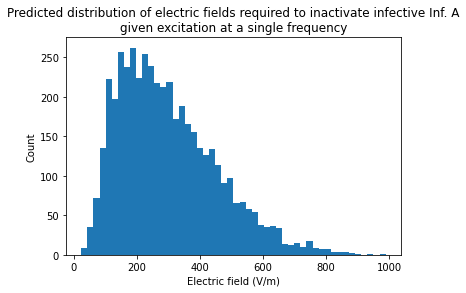
\includegraphics[width=\textwidth]{biology/output_35_1.png}
\end{figure}



\printbibliography[heading=none, title={}]





\end{document}

